% fixture: tikz/labels-pdftex
% oracle: pdflatex
% tier: T3
% engine: document
% specials: compare
% covers: nodes on paths: labels on --, -|, |-, to and rectangle (midway by default, pos=, near end), auto and swap, sloped (and turned not to be upside down), above and below, in a rotated scope, a coordinate on a line; nodes at the ends of a path and in \tikz, a cycle after a node; a line to a circle node's border; math in a node, text= under a scope's draw=, a trailing space, transform shape, font=\small
% issue: #320
\documentclass{article}
\usepackage{tikz}
\begin{document}
\noindent Labels:
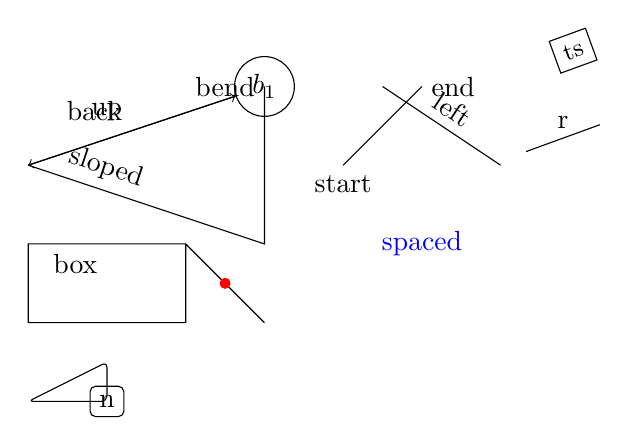
\begin{tikzpicture}[auto]
  \coordinate (a) at (0,0);
  \node[draw,circle] (b) at (3,1) {$b_1$};
  \draw[->] (a) -- node {up} (b);
  \draw[->] (b) to node[swap] {back} (a);
  \draw (a) -- node[sloped, above, pos=0.3] {sloped} (3,-1) |- node[near end] {bend} (b);
  \draw (0,-2) rectangle node {box} (2,-1) -- coordinate (m) (3,-2);
  \fill[red] (m) circle (2pt);
  \draw (4,0) node[below] {start} -- (5,1) node[right] {end};
  \begin{scope}[draw=red]
    \node[text=blue] at (5,-1) {spaced };
  \end{scope}
  \draw[rounded corners=2pt] (0,-3) -- (1,-3) node[draw] {n} -- (1,-2.5) -- cycle;
  \draw (6,0) -- node[sloped, above] {left} (4.5,1);
  \begin{scope}[rotate=20]
    \draw (6,-2) -- node[above] {r} (7,-2);
    \node[draw, transform shape, font=\small] at (7,-1) {ts};
  \end{scope}
\end{tikzpicture}
and \tikz \draw (0,0) node[left] {$x$} -- (1,0) node[right] {$y$}; after.
\end{document}
